\section{Moti Longitudinali}
Vengono ora analizzati i moti longitudinali del sistema, analisi che sarà successivamente impiegata per stabilizzare il sistema e per sviluppare un autopilota in grado di mantenere una determinata altitudine di volo.

Uno dei compiti del pilota di un velivolo è quello di mantenere una determinata quota, al fine di evitare potenziali collisioni con altri aeromobili.
Un pilota ben addestrato e attento è in grado di svolgere questo compito manualmente con una precisione di $\pm 50$ ft; per tale motivo i controllori del traffico aereo si aspettano che tale tolleranza venga rispettata.

Poiché questo compito richiede un elevato livello di attenzione e diligenza, gli aeromobili più sofisticati sono spesso dotati di un autopilota per il mantenimento della quota, così da ridurre il carico di lavoro del pilota.

\subsection{Ingressi e Uscite}

Il controllo dell'altitudine verrà effettuato agendo esclusivamente sugli equilibratori; la forza propulsiva non viene modificata dal controllore.

A tal fine, viene utilizzato un altimetro barometrico per la misura dell'altitudine del velivolo, strumento comunemente impiegato nei sistemi avionici per stimare la quota in base alla pressione atmosferica.

\begin{figure}[H]
    \centering
    \begin{tikzpicture}
        \node[draw,
            circle,
            minimum size=0.5cm,
        ] (sum) at (0,0){};

        % Controller
        \node [draw,
            minimum width=2.4cm,
            minimum height=1.2cm,
            right=1.5cm of sum
        ]  (controller) {$Controllore$};

        % System
        \node [draw,
            minimum width=2.4cm,
            minimum height=2.8cm,
            right=1.5cm of controller,
            yshift=0.8cm
        ]  (system) {$Sistema$};

        % Sensor block
        \node [draw,
            minimum width=2.4cm,
            minimum height=1.2cm,
            below right= 1cm and -0.25cm of controller
        ]  (sensor) {$Altimetro$};


        \draw[-stealth] (system.east) -- ++ (1.5,0)
        node[midway](output){}node[midway,above]{$z$};

        \draw[stealth-] (system.150) -- ++ (-1.5,0)
        node[midway,above]{$\delta_t$};

        \draw[-stealth] (controller.east) -- ++ (1.5,0);

        \draw[-stealth] (sum.east) -- ++ (1.5,0);
        \draw[stealth-] (sum.west) -- ++ (-1.25,0)
        node[midway,above]{$\delta_e$};

        \draw[-stealth] (sensor.west) -| (sum.south);

        \draw[-stealth] (output.center) |- (sensor.east);
    \end{tikzpicture}
\end{figure}

\renewcommand{\arraystretch}{1.2}
\begin{table}[H]
    \begin{tabularx}{\textwidth}{|c|X|}
        \hline
        \multicolumn{2}{|l|}{\textbf{Ingressi}}                                          \\
        \hline
        $\delta_e$ & angolo di deflessione degli equilibratori                           \\
        \hline
        \multicolumn{2}{|l|}{\textbf{Uscite}}                                            \\
        \hline
        $z$        & Variazione dell'altitudine rispetto al valore iniziale di 20.000 ft \\
        \hline
        \multicolumn{2}{|l|}{\textbf{Variabili di Stato}}                                \\
        \hline
        $u$, $w$   & componenti lungo $x_{FRD}$ e $z_{FRD}$ del vettore $\vec{V}_{FRD}$  \\
        $q$        & componente lungo $y_{FRD}$ del vettore $\vec{w}_{FRD}$              \\
        $\theta$   & angolo di beccheggio                                                \\
        $z$        & Variazione dell'altitudine rispetto al valore iniziale di 20.000 ft \\
        \hline
    \end{tabularx}
\end{table}

\subsection{Funzione di Trasferimento}
Utilizzando la funzione \texttt{ss2tf} di MATLAB sul modello di stato \eqref{eq:motoLongitudinale} si ottiene la funzione di trasferimento:

\begin{equation}
    \label{eq:trasferimentoLongitudinali}
    \begin{split}
        W_{\delta_e \rightarrow z}(s) & = \frac{32.7 s^3 + 7.0486 s^2 - 1035.7 s - 4.5535}{s^5 + 1.4722 s^4 + 1.6835 s^3 + 0.010443 s^2 + 0.00017507 s} \\
                                      & = 32.7\frac{(s + 0.0043964)(s - 5.5234)(s + 5.7345)}{s(s + 0.73303 \pm j1.0663)(s + 0.0030727 \pm j0.0097528)}
    \end{split}
\end{equation}

Dalla forma di Evans \cite{zampieri_dispensa_controlli}, riportata nella seconda riga, è possibile individuare i poli e gli zeri. In particolare sono presenti tre zeri, $s = -0.0043964, s = 5.5234, s = - 5.7345$, e cinque poli, $s = 0, s = -0.73303 \pm j1.0663, s = -0.0030727 \pm j0.0097528$

\begin{figure}[H]
    \centering
    \begin{minipage}{.48\textwidth}
        \centering
        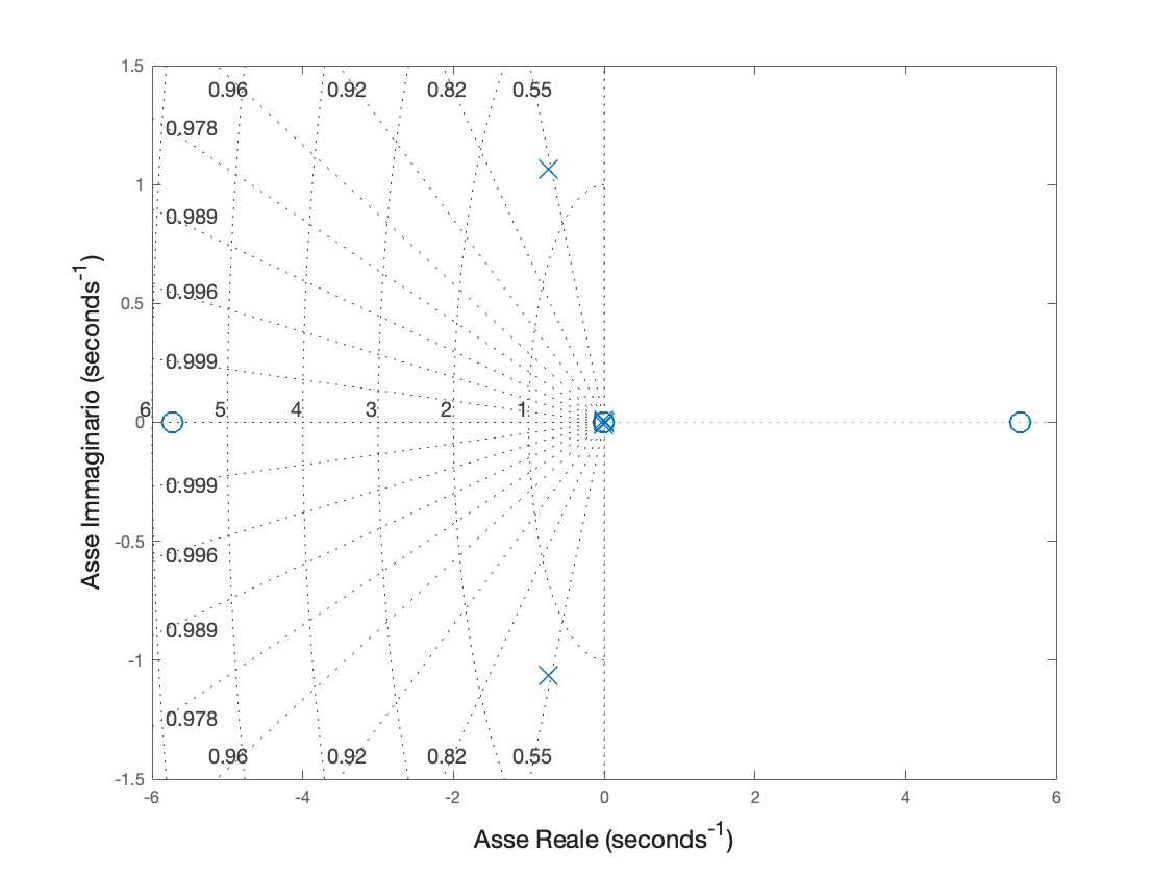
\includegraphics[width=1\linewidth]{Immagini/poli_longitudinali.pdf}
        \captionof{figure}{\texttt{pzplot} dei poli e degli zeri della funzione di trasferimento $W_{\delta_e \rightarrow z}(s)$}
    \end{minipage}
    \hspace{0.02\textwidth}
    \begin{minipage}{.48\textwidth}
        \centering
        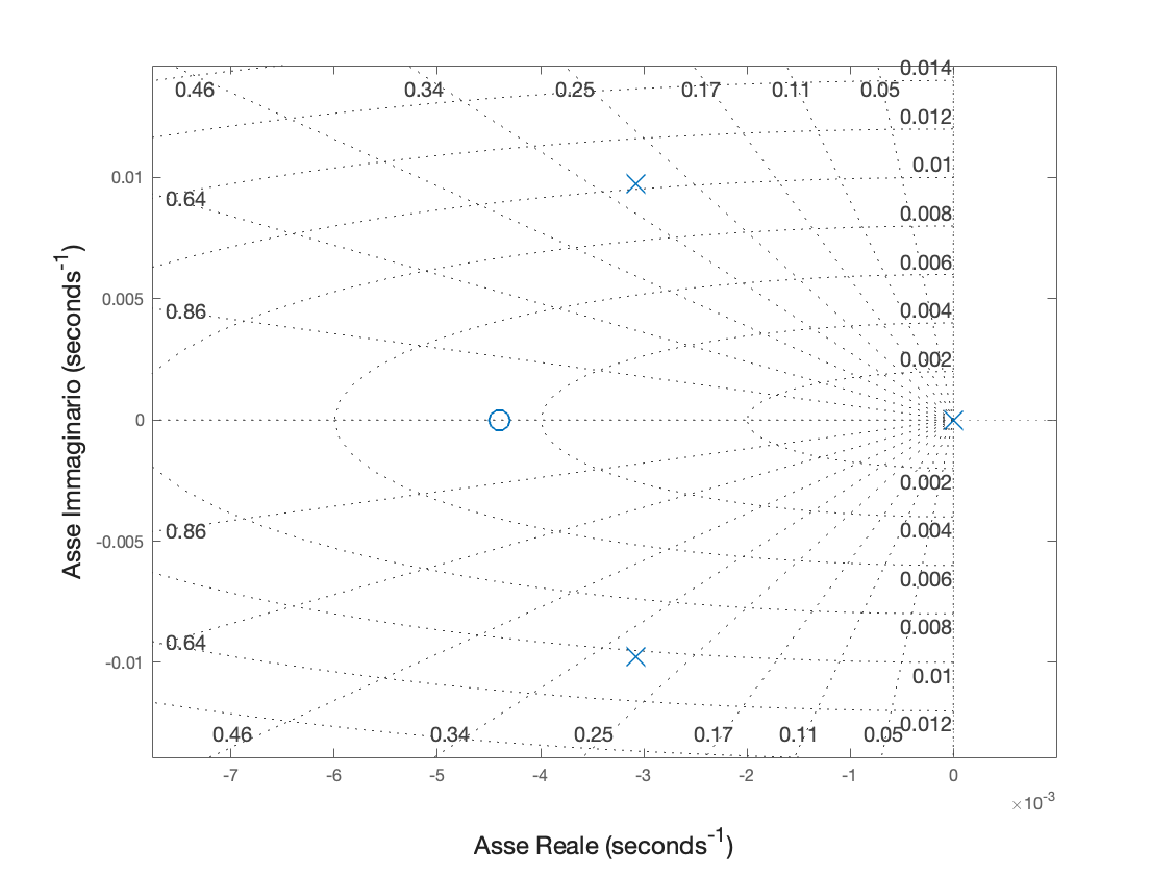
\includegraphics[width=1\linewidth]{Immagini/poli_longitudinali_detail.pdf}
        \captionof{figure}{Dettaglio del grafico vicino all'origine}
    \end{minipage}
\end{figure}


\subsection{Stabilità}

\subsubsection{Stabilità Rispetto alle Condizioni iniziali}

Come definito in \cite{zampieri_dispensa_controlli}:
\begin{sitemize}
    \item un sistema si dice \textbf{asintoticamente stabile} rispetto alle condizioni iniziali quando la sua risposta libera tende a 0: $\lim_{t\to\infty} y_l(t) = 0$.
    \item un sistema si dice \textbf{semplicemente stabile} rispetto alle condizioni iniziali quando la sua risposta libera è limitata : $\left|y_l(t)\right| < M \quad \forall t \geq 0$.
\end{sitemize}

Si può inoltre enunciare il seguente teorema:
\begin{sitemize}
    \item un sistema è \textbf{asintoticamente stabile} rispetto alle condizioni iniziali se e solo se tutte le radici del polinomio caratteristico del sistema ($p_1, p_2, \dots, p_n$) hanno parte reale negativa $Re[p_i] < 0$.
    \item un sistema è \textbf{semplicemente stabile} rispetto alle condizioni iniziali se e solo se tutte le radici del polinomio caratteristico del sistema ($p_1, p_2, \dots, p_n$) hanno parte reale negativa o uguale a $0$ $Re[p_i] \leq 0$.
\end{sitemize}

Il polinomio caratteristico del sistema si può trovare nel denominatore della funzione di trasferimento \eqref{eq:trasferimentoLongitudinali}:
\begin{equation*}
    s(s + 0.73303 \pm j1.0663)(s + 0.0030727 \pm j0.0097528)
\end{equation*}
Le sue radici hanno tutte parte reale minore o uguale a zero, è quindi possibile concludere che il sistema è semplicemente stabile rispetto alle condizioni iniziali.

\subsubsection{BIBO Stabilità}\label{subsubsec:bibo-instabile}

Come definito in \cite{zampieri_dispensa_controlli}:
\begin{sitemize}
    \item un sistema si dice \textbf{BIBO (Bounded Input-Bounded Output) stabile} se ad ogni ingresso limitato, il sistema genera una risposta forzata limitata.
\end{sitemize}

Viene inoltre enunciato il seguente teorema:
\begin{sitemize}
    \item un sistema è \textbf{BIBO stabile} se e solo se la sua funzione di trasferimento ha tutti i poli a parte reale negativa.
\end{sitemize}

Come per la stabilità rispetto alle condizioni iniziali, a causa della presenza di un polo in $s = 0$ a parte reale non negativa il sistema non è BIBO stabile.

L'instabilità del sistema è evidente osservando la risposta al gradino $\delta_e(t) = \delta^{-1}(t)$:

\begin{figure}[H]
    \centering
    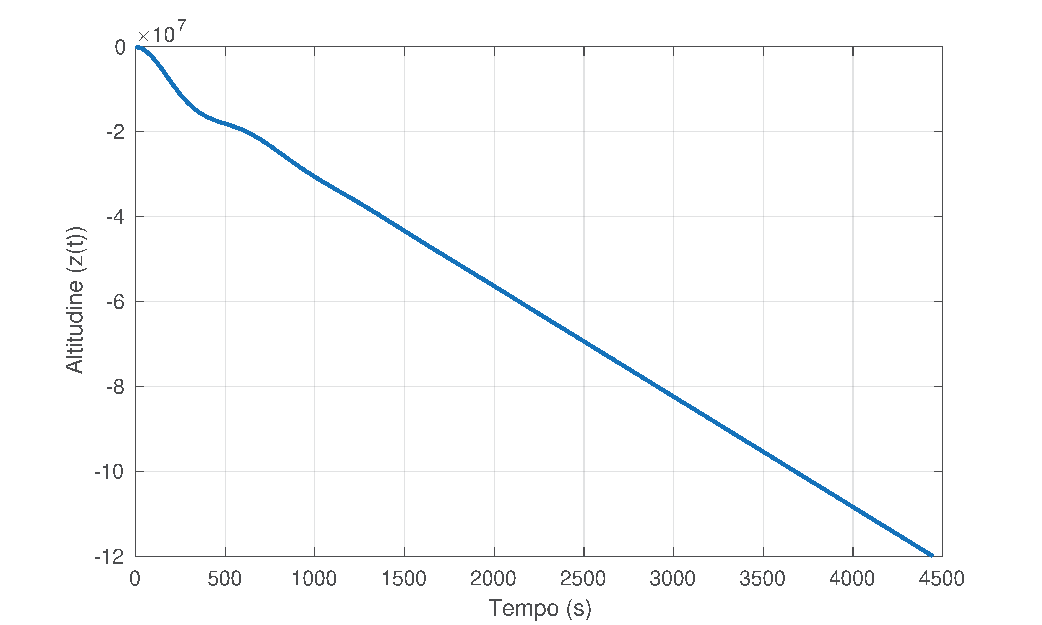
\includegraphics[width=0.65\linewidth]{Immagini/BIBO_instabile.pdf}
\end{figure}

\subsection{Modi Naturali}

La funzione di trasferimento evidenzia, oltre al polo in $s = 0$ che ha dominato la precedente analisi della stabilità, anche due altri poli complessi coniugati.

Un parametro che caratterizza la risposta dinamica di questi poli è il loro coefficiente di smorzamento.
Come si può notare dal grafico, a seconda del valore del coefficiente di smorzamento $\zeta$ si distinguono tre casi:
\begin{sitemize}
    \item quando $\zeta < 1$ il sistema è sottosmorzato, segue quindi un moto oscillatorio.
    \item quando $\zeta = 1$ il sistema è criticamente smorzato, il tempo per ritornare all'equilibrio è in questo caso minimo.
    \item quando $\zeta > 1$ il sistema è sovrasmorzato, ritorna all'equilibrio senza oscillazioni, ma impiega un tempo maggiore del caso precedente.
\end{sitemize}

\begin{figure}[H]
    \centering
    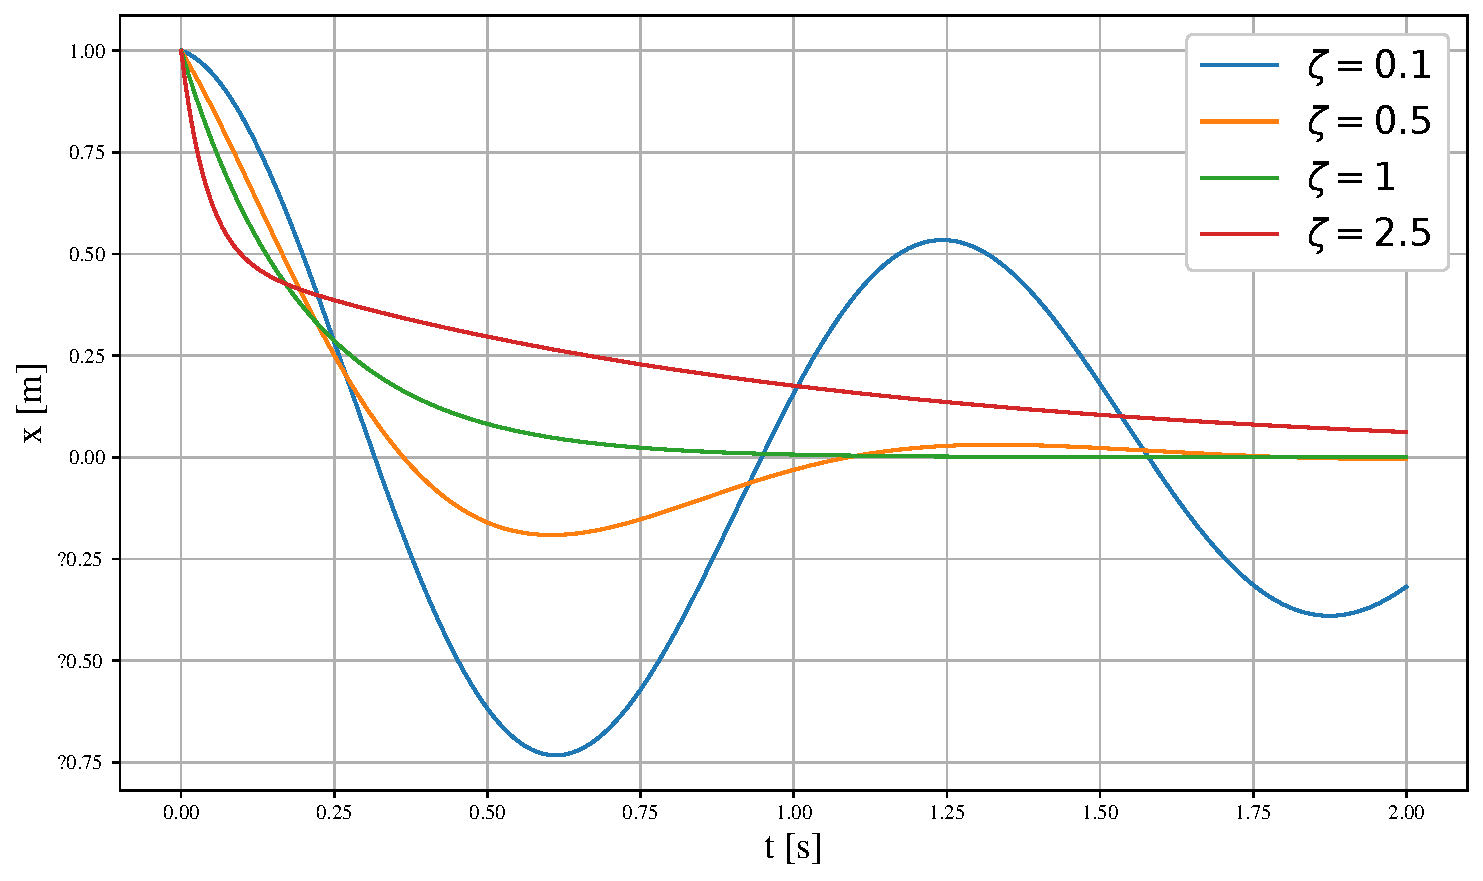
\includegraphics[width=0.65\linewidth]{Immagini/vibrazione_sistema.pdf}
    \caption{Vibrazione di un sistema massa-molla-smorzatore per diversi valori di $\zeta$}
\end{figure}

\subsubsection{Short-Period}\label{subsubsec:short_period}

Il modo associato ai poli in $-0.73303 \pm j1.0663$ è detto \textit{short-period} per la sua breve durata, esso avviene quando il velivolo in volo rettilineo simmetrico uniforme è soggetto ad una raffica di vento verticale o ad un impulso di $\delta_e(t)$.

Il coefficiente di smorzamento e la pulsazione naturale per i poli si calcolano come segue \cite{zampieri_dispensa_controlli}:
\begin{equation*}
    \zeta = - \frac{Re[p]}{\left|p\right|} = 0.5665 \qquad \omega_n = \left|p\right| = 1.2939rad/s
\end{equation*}

Il moto oscillatorio causato da questi poli è fortemente smorzato e quindi di breve durata.

\begin{figure}[H]
    \centering
    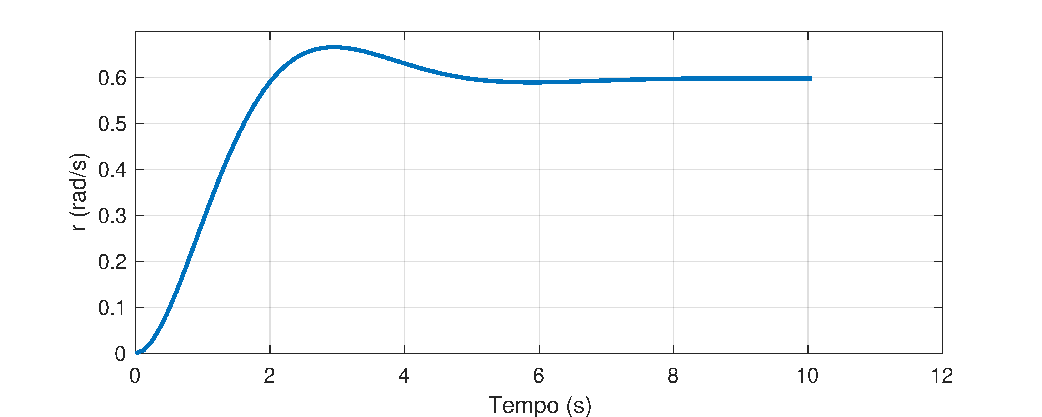
\includegraphics[width=0.7\linewidth]{Immagini/shortperiod_mode.pdf}
    \caption{Risposta impulsiva dei poli assiociati al modo \textit{short-period} assieme al polo nell'origine del Boeing 747 in esame}
\end{figure}

\subsubsection{Phugoid}

Il modo associato ai poli in $-0.0030727 \pm j0.0097528$ è detto \textit{phugoid}, esso avviene quando il velivolo in volo rettilineo simmetrico uniforme è soggetto ad una raffica di vento frontale.
Dopo la raffica di vento si innesca uno scambio tra energia potenziale e cinetica che si protrae per un lungo periodo di tempo.

\begin{figure}[H]
    \centering
    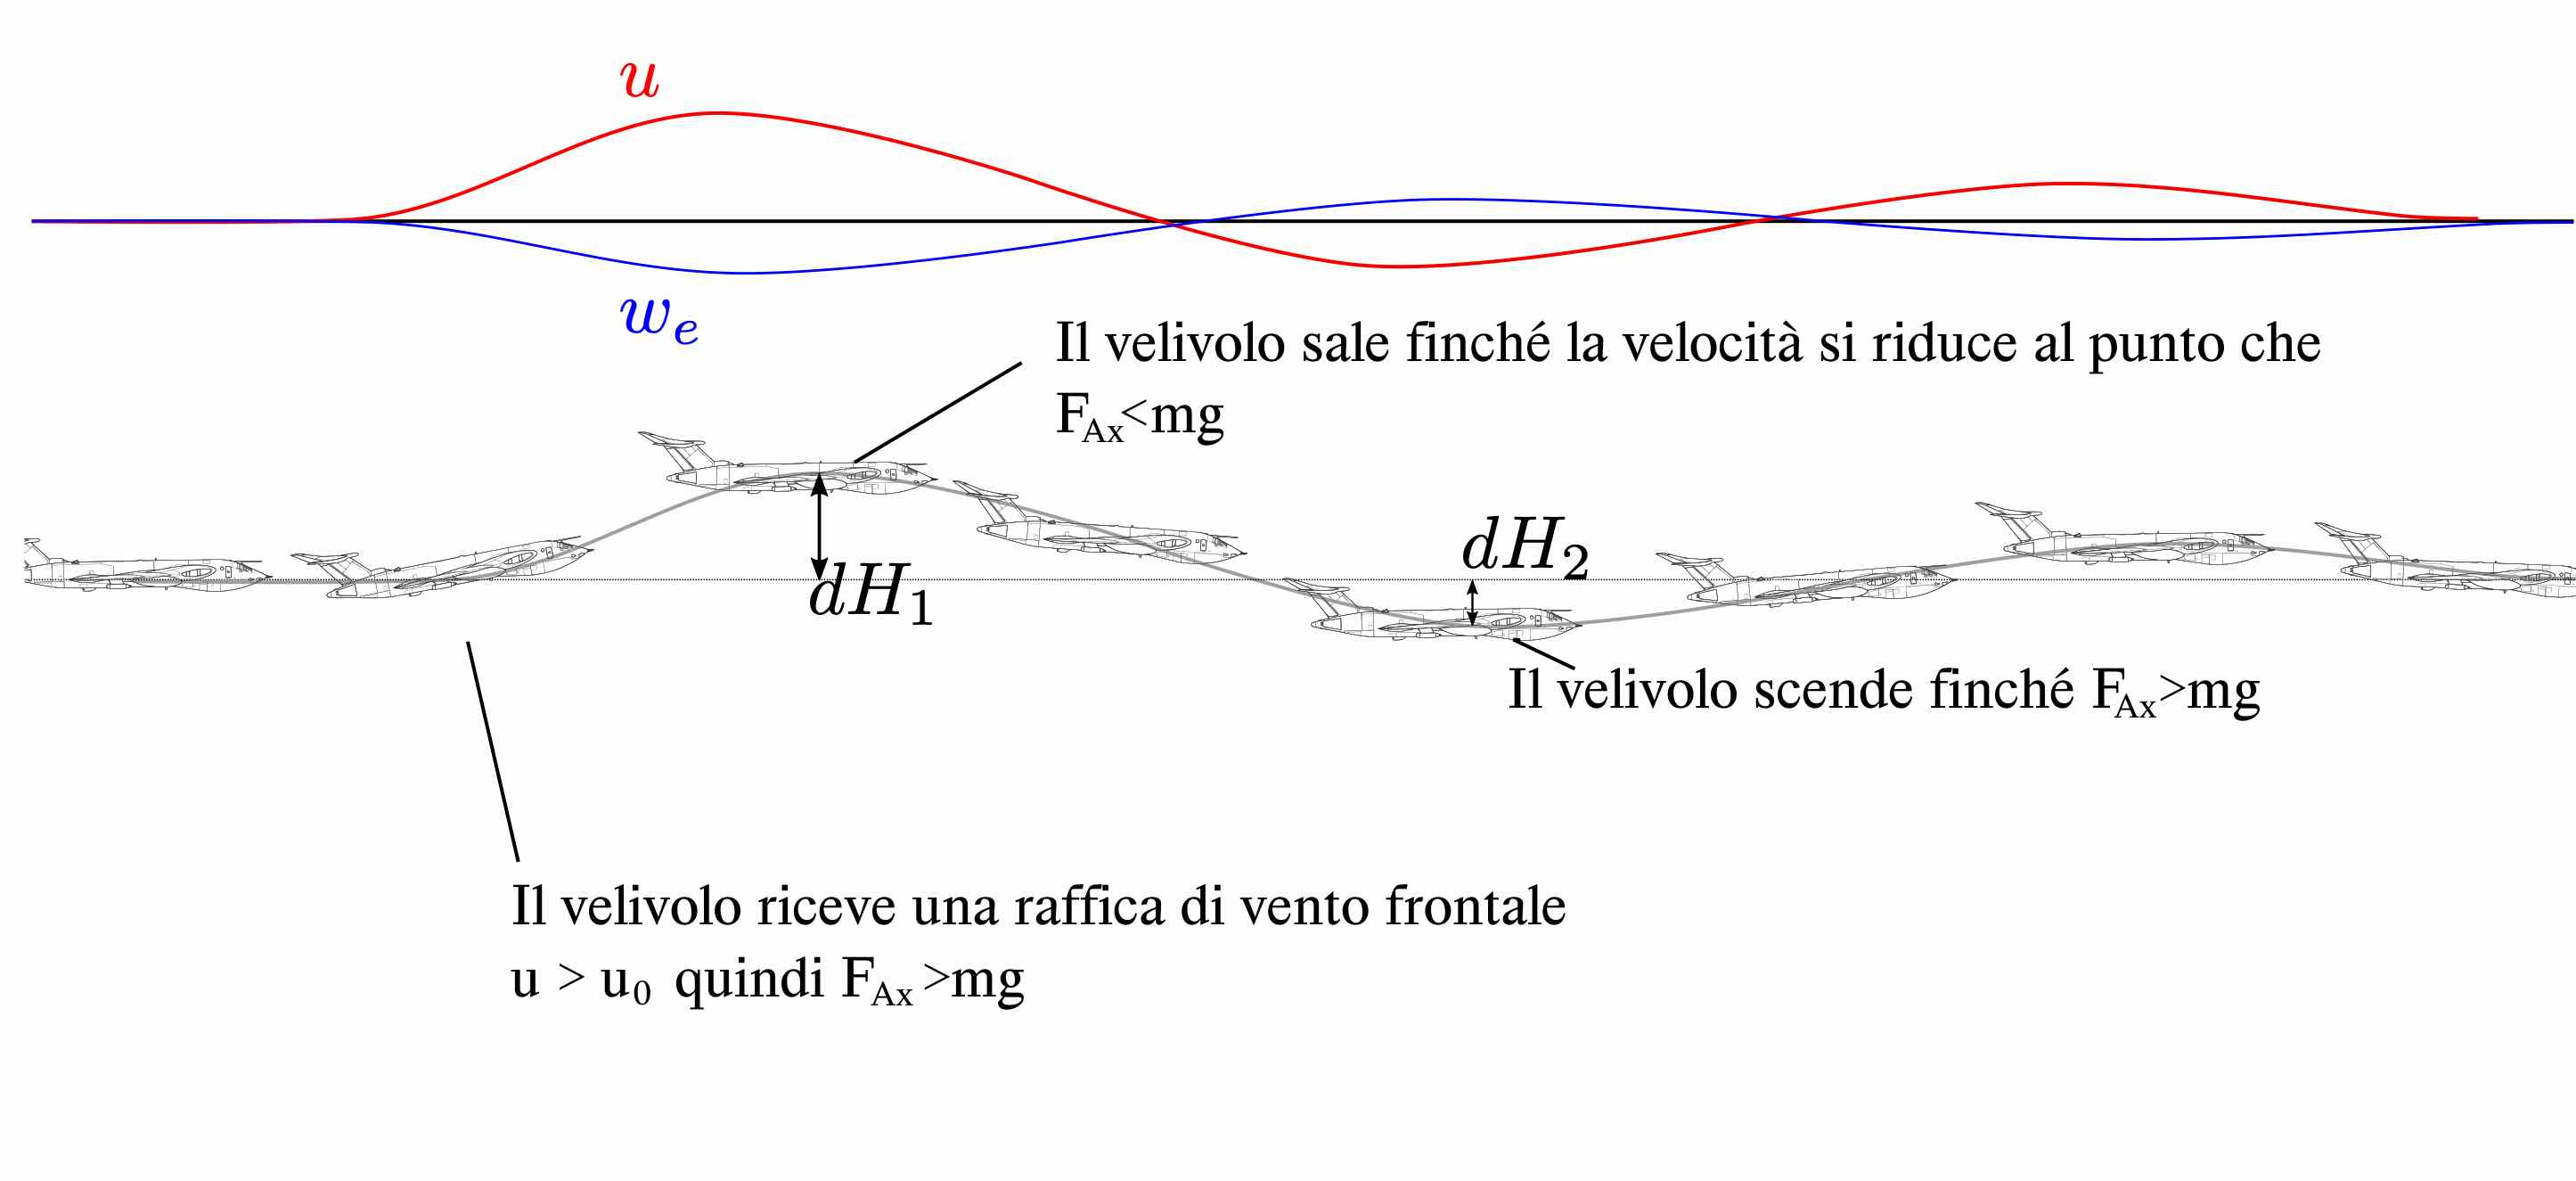
\includegraphics[width=0.9\linewidth]{Immagini/phugoid_mode_physics.jpg}
\end{figure}

In questo caso il coefficiente di smorzamento e la pulsazione naturale per i poli sono:
\begin{equation*}
    \zeta = - \frac{Re[p]}{\left|p\right|} = 0.3005 \qquad \omega_n = \left|p\right| = 0.01022rad/s
\end{equation*}

Si può notare che sia il coefficiente di smorzamento che la pulsazione naturale sono inferiori che nel modo precedente. Il tempo di assestamento è quindi molto maggiore, arrivando fino a 24 minuti per il Boeing 747 in esame.
\begin{figure}[H]
    \centering
    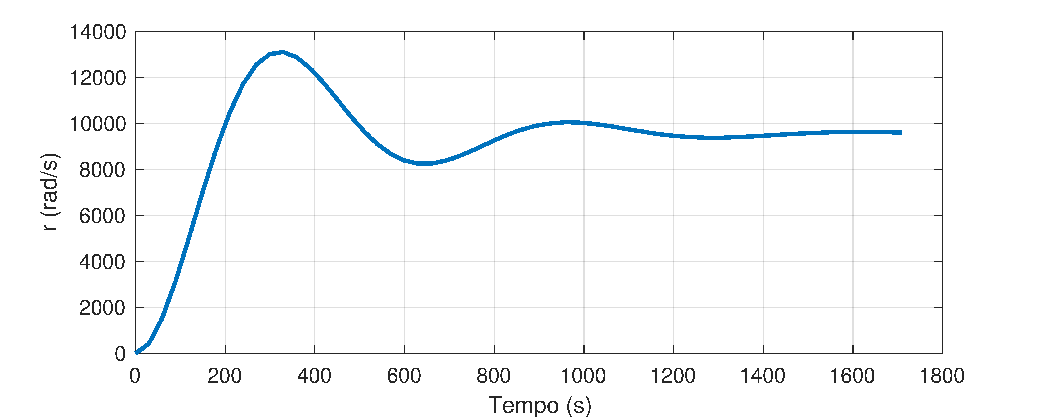
\includegraphics[width=0.7\linewidth]{Immagini/phugoid_mode.pdf}
    \caption{Risposta impulsiva dei poli associati al modo \textit{phugoid} assieme al polo nell'origine  del Boeing 747 in esame}
\end{figure}

